
%(BEGIN_QUESTION)
% Copyright 2006, Tony R. Kuphaldt, released under the Creative Commons Attribution License (v 1.0)
% This means you may do almost anything with this work of mine, so long as you give me proper credit

An electronic differential pressure transmitter with remote (chemical) seals is used to measure the level of liquid in this pressurized vessel.  The specific gravity of fill fluid in both remote seals is 0.934.  The range of liquid level measurement is 0 to 24 feet, and the output signal range is 4 to 20 mA.  Assume a calibration tolerance of +/- 0.25 percent.  Complete the following table of values for this transmitter.  Show the equations used to calculate all values given the percentage of span ($x$):

$$\includegraphics[width=15.5cm]{i00033x01.eps}$$

% No blank lines allowed between lines of an \halign structure!
% I use comments (%) instead, so that TeX doesn't choke.

$$\vbox{\offinterlineskip
\halign{\strut
\vrule \quad\hfil # \ \hfil & 
\vrule \quad\hfil # \ \hfil & 
\vrule \quad\hfil # \ \hfil & 
\vrule \quad\hfil # \ \hfil & 
\vrule \quad\hfil # \ \hfil & 
\vrule \quad\hfil # \ \hfil \vrule \cr
\noalign{\hrule}
%
% First row
Process & Percent of & $\Delta$ pressure & Output signal & Output signal & Output signal \cr
%
% Another row
level (ft) & span (\%) & sensed ("W.C) & ideal (mA) & min. (mA) & max. (mA) \cr
%
\noalign{\hrule}
%
% Another row
  & 0 &  &  &  &  \cr
%
\noalign{\hrule}
%
% Another row
  & 10 &  &  &  &  \cr
%
\noalign{\hrule}
%
% Another row
  & 25 &  &  &  &  \cr
%
\noalign{\hrule}
%
% Another row
  & 50 &  &  &  &  \cr
%
\noalign{\hrule}
%
% Another row
  & 75 &  &  &  &  \cr
%
\noalign{\hrule}
%
% Another row
  & 90 &  &  &  &  \cr
%
\noalign{\hrule}
%
% Another row
  & 100 &  &  &  &  \cr
%
\noalign{\hrule}
} % End of \halign 
}$$ % End of \vbox

\vskip 10pt

\noindent
{\bf Equations used:}

\vskip 20pt

Process level = 

\vskip 20pt

Pressure sensed = 

\vskip 20pt

Output signal (ideal) = 

\vskip 20pt

Output signal (min.) = 

\vskip 20pt

Output signal (max.) = 



\vfil 

\underbar{file i00033}
\eject
%(END_QUESTION)





%(BEGIN_ANSWER)

This is a graded question -- no answers or hints given!

%(END_ANSWER)





%(BEGIN_NOTES)

% No blank lines allowed between lines of an \halign structure!
% I use comments (%) instead, so that TeX doesn't choke.

$$\vbox{\offinterlineskip
\halign{\strut
\vrule \quad\hfil # \ \hfil & 
\vrule \quad\hfil # \ \hfil & 
\vrule \quad\hfil # \ \hfil & 
\vrule \quad\hfil # \ \hfil & 
\vrule \quad\hfil # \ \hfil & 
\vrule \quad\hfil # \ \hfil \vrule \cr
\noalign{\hrule}
%
% First row
Process & Percent of & $\Delta$ pressure & Output signal & Output signal & Output signal \cr
%
% Another row
level (ft) & span (\%) & sensed ("W.C.) & ideal (mA) & min. (mA) & max. (mA) \cr
%
\noalign{\hrule}
%
% Another row
0  & 0 & -269.0 & 4 & 3.96 & 4.04 \cr
%
\noalign{\hrule}
%
% Another row
2.4  & 10 & -228.4 & 5.6 & 5.56 & 5.64 \cr
%
\noalign{\hrule}
%
% Another row
6  & 25 & -167.5 & 8 & 7.96 & 8.04 \cr
%
\noalign{\hrule}
%
% Another row
12  & 50 & -66.01 & 12 & 11.96 & 12.04 \cr
%
\noalign{\hrule}
%
% Another row
18  & 75 & +35.49 & 16 & 15.96 & 16.04 \cr
%
\noalign{\hrule}
%
% Another row
21.6  & 90 & +96.38 & 18.4 & 18.36 & 18.44 \cr
%
\noalign{\hrule}
%
% Another row
24  & 100 & +137.0 & 20 & 19.96 & 20.04 \cr
%
\noalign{\hrule}
} % End of \halign 
}$$ % End of \vbox

\vskip 10pt

Process level = (Percent of Span) $\times$ 24 ft

\vskip 10pt

Pressure sensed = $\left( (\hbox{Level} \times 12) \times {88 \over 62.4} \right) - (24 \times 12 \times 0.934)$

\vskip 10pt

Output signal (ideal) = (Percent of Span) $\times$ 16 mA + 4 mA 

\vskip 10pt

Output signal (min.) = (Percent of Span) $\times$ 16 mA + 4 mA - (0.25\% $\times$ 16 mA) 

\vskip 10pt

Output signal (max.) = (Percent of Span) $\times$ 16 mA + 4 mA + (0.25\% $\times$ 16 mA) 

\vskip 10pt



%INDEX% Calibration: table, level transmitter
%INDEX% Measurement, level: calibration table

%(END_NOTES)


